\chapter{A Grand Apparatus}\label{ch:lhc_cms}
\begin{aquote}{Fran\c{c}ois Englert, CMS: The Art of Science, 2016}
    A glance at the ATLAS and CMS detectors at CERN reveals their beauty...
    These detectors are the modern cathedrals of the rational world created by scientists, experimentalists, and theoreticians. 
\end{aquote}
\section{The Large Hadron Collider}
The Large Hadron Collider (LHC) is the largest particle accelerator ever built. 
Its most striking feature is a 27 km ring (Fig.~\ref{fig:lhc_pics}) buried 175 m beneath the Franco-Swiss border in which two beams of protons, after going through several smaller stages, are accelerated to 99.9999991\% of the speed of light in opposite directions. 
The beams are steered by thousands of magnets placed along the circumference of the ring. 
At various points, the proton beams are directed towards each other, allowing the protons to collide. 
These collision points are surrounded by enormous, multi-layered particle detectors which record snapshots of the collisions. 

The protons are accelerated in bunches (with roughly 115 billion protons per bunch) spaced apart by 25 nanoseconds, so when the two beams are focused together (called a ``bunch crossing''), over 200 billion protons are brought very close together, yet only a small portion of them collide. 
During ``Run 2'' of the LHC, from 2016 to 2018, there were 30 proton-proton collisions per bunch crossing on average, with only a single ``interesting'' collision (the ``primary vertex'') amongst them. % TODO: define pileup somehow, citation needed, plot or something of pileup needed
Nevertheless, the thirty simultaneous collisions produce, together, thousands of subatomic particles. 
Therefore, particle detectors on the LHC must be able to resolve the particles from the primary vertex amongst the many others produced by the pileup---all within the 25 ns between bunch crossings. % Add some metaphor or something here to sell the scale maybe; how fast _is_ 25 ns?? (something that shows it's really really fast)

\begin{figure}[htb]
    \centering
    \subfloat{\includegraphics[width=0.465\textwidth]{fig/lhc/lhc_complex.png}}\quad
    \subfloat{\includegraphics[width=0.435\textwidth]{fig/lhc/cern_aerial_view.jpg}}
    \caption{
        The LHC complex illustrated in detail (right) and from a ``bird's eye'' perspective (left). 
    }
    \label{fig:lhc_pics}
\end{figure}

\section{The Compact Muon Solenoid}
\begin{figure}[htb]
    \centering
    \includegraphics[width=0.9\textwidth]{fig/cms/cms_labeled.jpg}
    \caption{
        Lorem ipsum.
    }
    \label{fig:cms_labeled}
\end{figure}
\subsection{Superconducting solenoid}
\subsection{Silicon tracker}
\subsection{Electromagnetic calorimeter}
\subsection{Hadronic calorimeter}
\subsection{Muon chambers}
% Overview: "Compact" "Muon" "Solenoid"?
%    - i.e. what is it supposed to do?
%    - show diagram from UChicago proposal of the generalized particle layers
% Explain each layer
%    - mention russia shells --> calorimeter
\begin{figure}[htb]
    \centering
    \subfloat{\includegraphics[width=0.465\textwidth]{fig/cms/cms_picture1.jpg}}\quad
    \subfloat{\includegraphics[width=0.435\textwidth]{fig/cms/cms_picture2.jpg}}
    \caption{
        The Compact Muon Solenoid in all of its glory, with one of the endcaps separated from the main body of the experiment, pictured from the top (left) and side (right). 
    }
    \label{fig:cms_pics}
\end{figure}

\begin{figure}[htb]
    \centering
    \subfloat{\includegraphics[width=0.482\textwidth]{fig/cms/cms_picture3.jpg}}\quad
    \subfloat{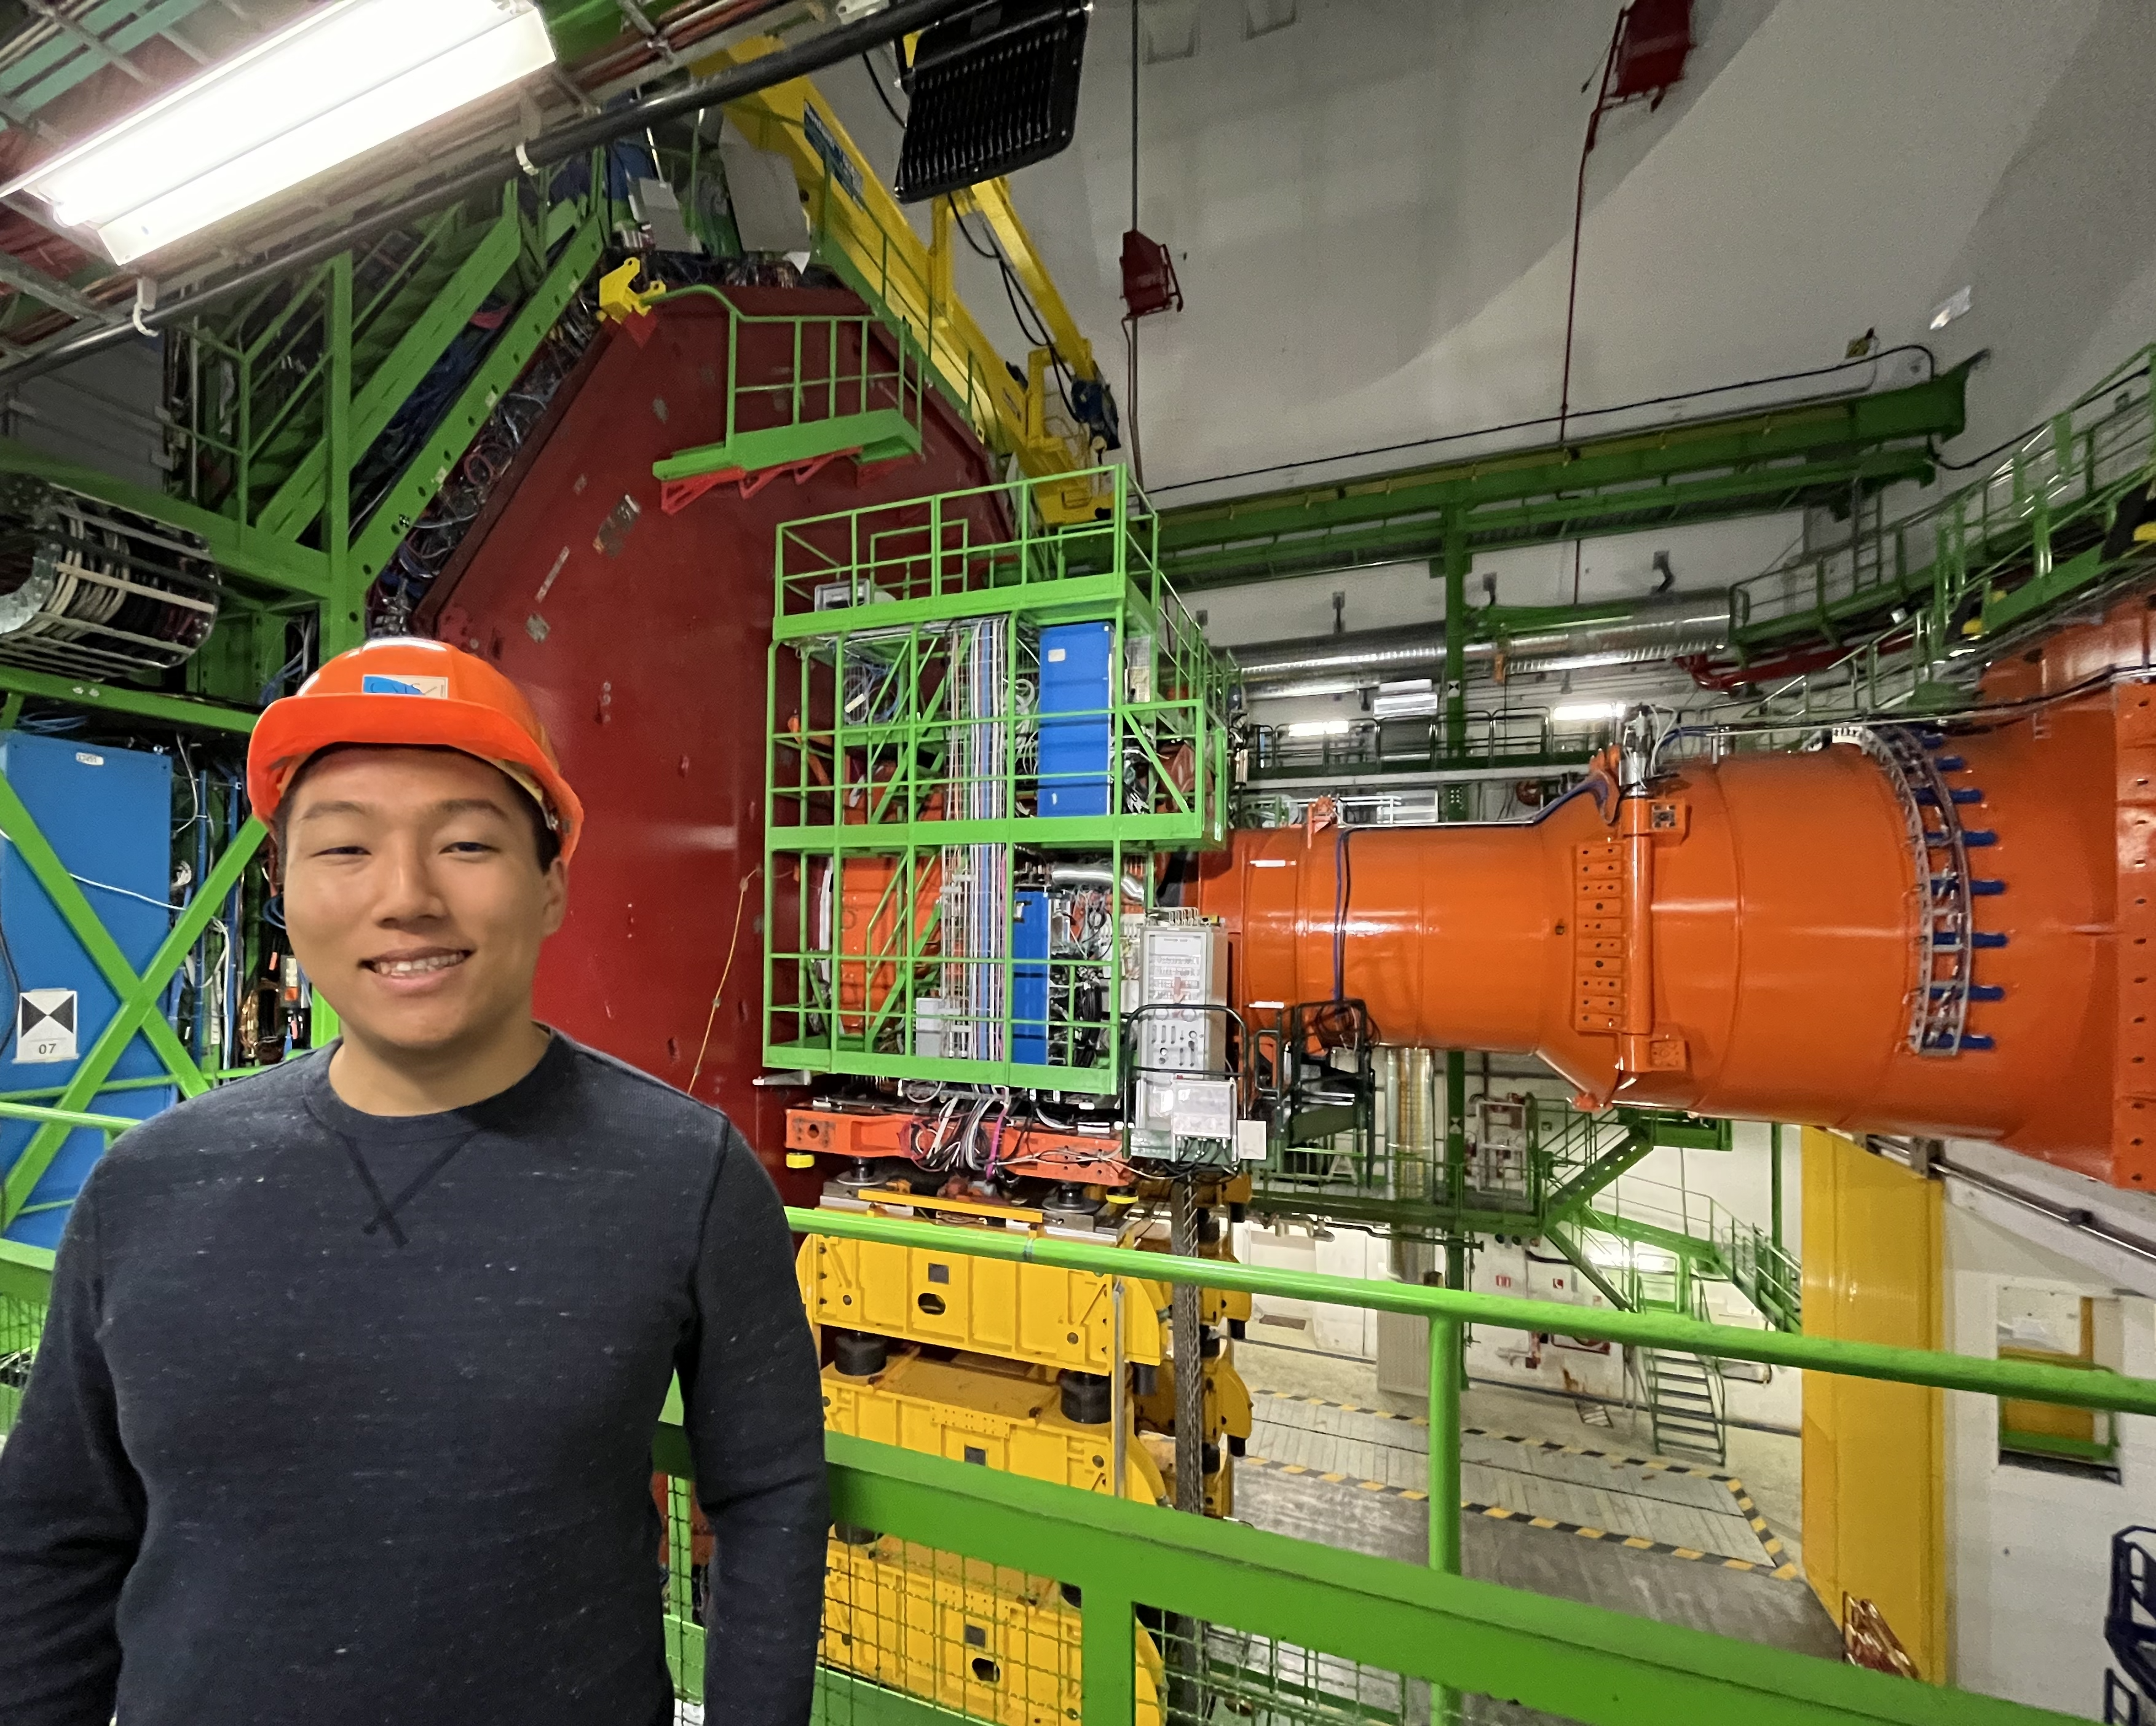
\includegraphics[width=0.4\textwidth]{fig/cms/cms_jguiang.jpg}}
    \caption{
        The Compact Muon Solenoid in the closed configuration, pictured from the top (left) and side (right).
    }
    \label{fig:cms_jguiang}
\end{figure}
\section{The high lumonisity era}
% What is HL?
%    - show pileup plots, maybe side AND 3D volume
% What benefits does it bring?
%    - Find some papers...
% What challenges does it bring?
%    - Show CPU/Data volume plots
